\documentclass[10pt]{article}
\usepackage[french]{babel}
\usepackage[utf8]{inputenc}
\usepackage[T1]{fontenc}
\usepackage{amsmath}
\usepackage{amsfonts}
\usepackage{amssymb}
\usepackage[version=4]{mhchem}
\usepackage{stmaryrd}
\usepackage{graphicx}
\usepackage[export]{adjustbox}
\graphicspath{ {./images/} }
\usepackage{bbold}

\title{TP1 Analyse numérique ( \(\Delta_{1}, K_{1}\) et \(\Sigma_{1}\) ) }

\author{Ibrahim ALAME}
\date{}


\begin{document}
\maketitle
26/02/2025

\section*{1 Problème de tir}
On reprend ici le dernier exemple du cours (chapitre 2). On lance un projectile de masse \(m\) avec une vitesse initiale \(\overrightarrow{v_{0}}\) faisant un angle \(\alpha\) avec l'axe horizontale. Le plan de tir est porté par un système d'axes ( \(O ; x, y\) ).\\
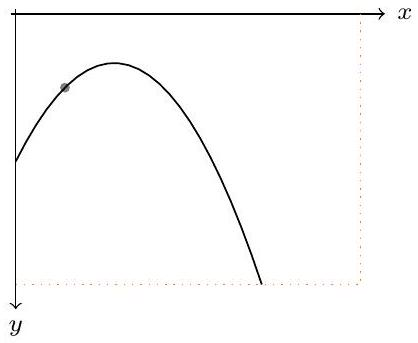
\includegraphics[max width=\textwidth, alt={}, center]{c65abac2-45d0-490f-87c5-f8506fdc2a1b-1_343_418_1065_852}

L'équation différentielle du mouvement \(\frac{\mathrm{d}^{2} M}{\mathrm{~d} t^{2}}=\vec{g}\) s'écrit en coordonnées \(x, y\) de M :

\[
\left\{\begin{array}{l}
x^{\prime \prime}=0 \\
y^{\prime \prime}=g
\end{array}\right.
\]

On pose \(z_{0}=x, z_{1}=y, z_{2}=x^{\prime}, z_{3}=y^{\prime}\). On a alors

\[
\left\{\begin{array}{c}
z_{0}^{\prime}=z_{2} \\
z_{1}^{\prime}=z_{3} \\
z_{2}^{\prime}=0 \\
z_{3}^{\prime}=g
\end{array}\right.
\]

On a donc un problème de Cauchy :

\[
\left\{\begin{array}{l}
Z^{\prime}=f(Z) \\
Z_{0} \text { donné }
\end{array}\right.
\]

où \(Z=\left[z_{0}, z_{1}, z_{2}, z_{3}\right], f(Z)=\left[z_{2}, z_{3}, 0, g\right]\) et \(Z_{0}=\left[x_{0}, y_{0}, v_{0} \cos (\alpha), v_{0} \sin (\alpha)\right]\)\\
Le schéma d'Euler s'écrit :

\[
\left\{\begin{array}{l}
Z_{k+1}=Z_{k}+h f\left(Z_{k}\right) \\
Z_{0}=[10,200,50 \cos (\pi / 3),-50 \sin (\pi / 3)]
\end{array}\right.
\]

où \(h=0.1 s\) et \(g=9.81 \mathrm{~m} / \mathrm{s}^{2}\).\\
Le programme suivant applique la méthode d'Euler pour résoudre numériquement l'équation différentielle du problème et affiche le résultat en animation graphique dans une fenêtre tkinter de hauteur \(H=750 \mathrm{px}\) et de largeur \(W=750 \mathrm{px}\).

Copiez et exécutez ce code :

\begin{verbatim}
from tkinter import *
import numpy as np
# coordonnees initiales
x0, y0 = 10, 200
# vitesse initiale
alpha=np.pi/3
VO=50
# 'pas' du temps
h=0.1
z=np.array([x0,y0,V0*np.cos(alpha),-V0*np.sin(alpha)])
def f(z):
    return np.array([z[2],z[3],0,9.81])
def Euler():
    global z
    z=z+h*f(z)
    # deplacement de la balle a la nouvelle position
    can1.coords(balle, z[0], z[1], z[0] + 30, z[1] + 30)
    # La fenetre fen1 est actualisee en executant la
    # fonction Euler toutes les 10 millisecondes
    fen1.after(10, Euler)
# =====================
# Creation de la fenetre principale :
fen1 = Tk()
fen1.title("Probleme de tir")
# creation du canvas :
H=W=750
can1 = Canvas(fen1, bg='dark grey', height=H, width=W)
can1.pack()
# creation de la balle
balle = can1.create_oval(x0, y0, x0 + 30, y0 + 30, width=2, fill='red')
# Lancement de la fonction Euler
Euler()
# demarrage de la boucle principale:
fen1.mainloop()
\end{verbatim}

Nous voulons que la balle rebondisse sur les bords de la fenêtre. Pour cela, à chaque fois que la boule touche un mur il faut inverser la vitesse normale. Par exemple : Si \(z_{1}<0\) ou \(z_{1}>H\) alors \(z_{3}=-z_{3}\).

Compléter le programme pour que la balle rebondisse aux 4 bords indéfiniment. Faites tourner\\
le programme pendant plus d'une minute. Que remarquez-vous? Modifiez le programme en passant à la méthode de Heun :

\[
\left\{\begin{array}{l}
Z_{k+1}=Z_{k}+\frac{h}{2}\left[f\left(Z_{k}\right)+f\left(Z_{k}+h f\left(Z_{k}\right)\right)\right] \\
Z_{0}
\end{array}\right.
\]

Commentez le résultat obtenu.\\
Dans cette question nous supposons que le projectile est soumis à une force de frottement proportionnelle à la vitesse, \(\vec{f}=-k \vec{v}\). Écrire l'équation différentielle et le problème de Cauchy du mouvement. Actualiser le programme pour simuler la trajectoire réaliste de la balle en prenant \(k=0.02\).

\section*{2 Mouvement des planètes}
\subsection*{2.1 Soleil-Terre}
Nous savons que le mouvement d'un point matériel dans un champs à force centrale a lieu dans un plan. Le plan de mouvement est d'origine au coin gauche supérieur de l'écran conformément à la convention informatique. Le soleil occupe la position fixe \(S(a, b)\). La terre est repérée par son centre \(T(x, y)\) ses coordonnées sont solution de l'équation différentielle : \(\frac{\mathrm{d}^{2} T}{\mathrm{~d} t^{2}}=\frac{G M_{s}}{r^{2}} \vec{u}\) où \(r=S T\) et \(\vec{u}=\frac{\overrightarrow{S T}}{S T}, G\) est la constante de gravitation \(G=6.67 \times 10^{-11} S I\) et \(M_{s}\) est la masse du soleil \(M s=1.989 \times 10^{30} \mathrm{~kg}\).\\
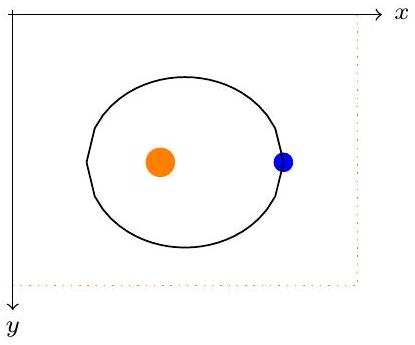
\includegraphics[max width=\textwidth, alt={}, center]{c65abac2-45d0-490f-87c5-f8506fdc2a1b-3_345_415_1284_855}

Comme pour le problème de tir, on pose \(z_{0}=x, z_{1}=y, z_{2}=x^{\prime}, z_{3}=y^{\prime}\). On a alors

\[
\left\{\begin{array}{l}
z_{0}^{\prime}=z_{2} \\
z_{1}^{\prime}=z_{3} \\
z_{2}^{\prime}=-G M_{s} \frac{z_{0}-a}{{\sqrt{\left(z_{0}-a\right)^{2}+\left(z_{1}-b\right)^{2}}}^{3}} \\
z_{3}^{\prime}=-G M_{s} \frac{z_{1}-b}{{\sqrt{\left(z_{0}-a\right)^{2}+\left(z_{1}-b\right)^{2}}}^{3}}
\end{array}\right.
\]

Le programme suivant est une simulation du mouvement de la terre autour du soleil. Copiez, exécuter et commenter ce programme. Améliorer la résolution numérique en utilisant la méthode d'Euler amélioré puis la méthode de Range et Kutta.

\begin{verbatim}
from tkinter import *
import numpy as np
\end{verbatim}

\begin{verbatim}
def f(z):
    r = np.sqrt((z[0] - a) ** 2 + (z[1] - b) ** 2)
    A = G * Ms / r ** 2
    Ax, Ay = -A * (z[0] - a) / r, -A * (z[1] - b) / r
    return np.array([z[2], z[3], Ax , Ay ])
def Euler():
    global z, h
    z=z+h*f(z)
    x1,y1 = z[0] // k, z[1] // k
    can1.coords(terre, x1, y1, x1 + 20, y1 + 20)
    fen1.after(1, Euler)
# ========== Programme principal ===========
H, W = 4.0E11, 4.0E11
a, b = W / 2, H / 2 # centre de la terre
k = 4.0E8
# coordonnees initiales
x0, y0 = a + 1.47E11, H / 2
# vitesse initiale
v0 = 30200
alpha = np.pi / 2
Ms = 1.989E30
G = 6.67E-11
z = np.array([x0, y0, VO * np.cos(alpha), -VO * np.sin(alpha)])
# 'pas' du temps
h = 3600
fen1 = Tk()
fen1.title("Terre-Soleil")
can1 = Canvas(fen1, bg='dark grey', height=H // k, width=W // k)
can1.pack()
x1, y1 = z[0] // k, z[1] // k
terre = can1.create_oval(x1,y1 , x1 + 20, y1 + 20, width=2, fill='blue')
R = 6963400000
R=R*5
x1, y1=(a - R) // k, (b - R) // k
x2, y2=(a+R) // k, (b + R) // k
soleil = can1.create_oval(x1, y1, x2, y2, width=2, fill='yellow')
# Lancement de la fonction Euler
Euler()
# Boucle principale:
fen1.mainloop()
\end{verbatim}

\subsection*{2.2 Soleil-Terre-Lune}
Les équations différentielles de la dynamique du système (S-T-L) : soleil \(S(a, b)\), terre \(T\left(x_{t}, y_{t}\right)\) et lune \(L\left(x_{\ell}, y_{\ell}\right)\), s'écrivent :

\[
\left\{\begin{array}{l}
\frac{\mathrm{d}^{2} T}{\mathrm{~d} t^{2}}=-\frac{G M_{s}}{r_{1}^{2}} \vec{u}_{1}-\frac{G M_{l}}{r_{2}^{2}} \vec{u}_{2} \\
\frac{\mathrm{~d}^{2} L}{\mathrm{~d} t^{2}}=-\frac{G M_{s}}{r_{3}^{2}} \vec{u}_{3}+\frac{G M_{t}}{r_{2}^{2}} \vec{u}_{2}
\end{array}\right.
\]

On pose \(z_{0}=x_{t}, z_{1}=y_{t}, z_{2}=x_{t}^{\prime}, z_{3}=y_{t}^{\prime}, z_{4}=x_{\ell}, z_{5}=y_{\ell}, z_{6}=x_{\ell}^{\prime}, z_{7}=y_{\ell}^{\prime}\). Préciser la fonction \(f: \mathbb{R}^{8} \rightarrow \mathbb{R}^{8}\) de la formulation de Cauchy : \(Z^{\prime}=f(Z)\) du système (S-T-L).

\begin{enumerate}
  \item Écrire une nouvelle version du programme précédent permettant d'étudier le mouvement de la terre et de la lune autour du soleil.
  \item Vérifier que l'année est \(\simeq 365\) jours et que le mois est \(\simeq 30\) jours.\\
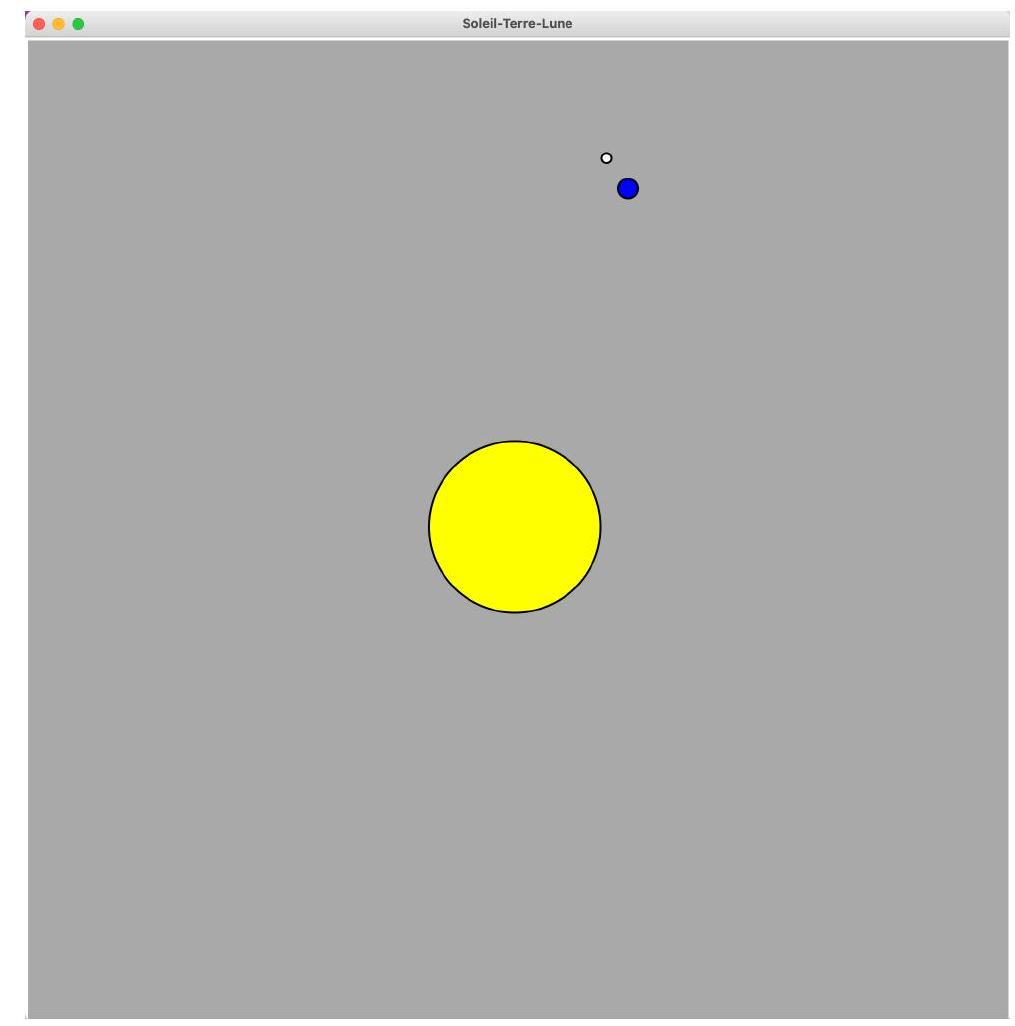
\includegraphics[max width=\textwidth, alt={}, center]{c65abac2-45d0-490f-87c5-f8506fdc2a1b-5_1026_1015_867_545}
\end{enumerate}

\end{document}